\documentclass[11pt]{report}
% this one apparently fixes the < and > chars
\usepackage[T1]{fontenc}
\usepackage{subfigure}
\usepackage{times}
\usepackage{tabularx}
% why did we need this?
%\usepackage{verbatim}
% make all captions small and slanted
\usepackage[small,sl]{caption}
\usepackage{fullpage}
%\usepackage{epsf}
\usepackage{epsfig}
% add nifty DRAFT watermark thingy in PS
%\usepackage{draftcopy}

\def\VERSION {1.2}
\def\DEFAULTPORT {6665}

\begin{document}
\setcounter{page}{0}
\pagenumbering{roman}

\titlepage

\begin{tabular}{lcr}
  \begin{tabular}{c}
	Player/Stage project\\
        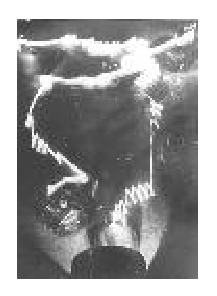
\includegraphics{notext_ps_logo}
   \end{tabular}
  &
  \hspace{5cm}
  &
  \begin{tabular}{r}
    {\bf USC Robotics Laboratory}\\
    University of Southern California\\
    Los Angeles, California, USA\\
    \vspace*{2em}\\
    {\bf Information Sciences Laboratory}\\
    HRL Laboratories\\
    Malibu, California, USA\\
  \end{tabular}
\end{tabular}

\vspace{5cm}
\centerline{\huge{Player C++ Client Library}}
\vspace{0.5cm}
\centerline{\large{Version \VERSION\ Reference Manual}}
\vspace{2cm}

\centerline{\large Brian P. Gerkey\\ Richard T. Vaughan\\ Andrew Howard}
\vspace{1cm}
%\centerline{Technical Report IRIS-00-392}
%\centerline{{\tt http://iris.usc.edu/${}_{\tilde{}}$\,irislib}}
%\vspace{1cm}
%\centerline{This report may not contain the most current documentation on}
%\centerline{Player.  For the latest documentation, consult the Player homepage:}
%\centerline{{\tt http://fnord.usc.edu/player}}

\centerline{This document may not contain the most current documentation on}
\centerline{Player.  For the latest documentation, consult the Player homepage:}
\centerline{{\tt http://robotics.usc.edu/player}}

\vspace{4cm}

\centerline{\today}

% reset page number to start with 1
\setcounter{page}{0}
\pagenumbering{arabic}

\chapter{Overview}

The C++ client ({\tt client\_libs/c++}) is generally the 
most comprehensive library, since it
is used to test new features as they are implemented in the server.
It is also the most widely used client library and thus the best 
debugged.  Having said that, this client is not perfect, but should
be straightforward to use by anyone familiar with C++.

The C++ library is built on a "service proxy" model in which the client
maintains local objects that are proxies for remote services.  There are
two kinds of proxies: the special server proxy {\tt PlayerClient} and the
various device-specific proxies.  Each kind of proxy is implemented as
a separate class.  The user first creates a {\tt PlayerClient} proxy and 
uses it to establish a connection to a Player server.  Next, the proxies
of the appropriate device-specific types are created and initialized
using the existing {\tt PlayerClient} proxy.
To make this process concrete, consider the following simple example 
(for clarity, we omit some error-checking):

{\small
\begin{verbatim}
  int main(int argc, char **argv)
  { 
    /* Connect to Player server on "localhost" at default port */
    PlayerClient robot("localhost");
    /* Request access to the ptz camera */
    PtzProxy zp(&robot,0,'a');

    int dir = 1;
    for(;;)
    {
      if(robot.Read())
        exit(1);
  
      // print out current camera state
      zp.Print();
  
      if(zp.pan > 80 || zp.pan < -80)
        dir = -dir;
  
      zp.SetCam(zp.pan + dir * 5,zp.tilt,zp.zoom);
    }

    // won't actually get here, but...
    robot.Disconnect();
  }
\end{verbatim}
}

This program will continuously pan the pan-tilt-zoom camera unit left and
right\footnote{Well, not exactly.  A little extra code is required to handle
the physical camera because it pans rather slowly; see 
{\tt examples/c++/ptz.cc} for the details.}.  First, a {\tt PlayerClient}
proxy is created, using the default constructor to connect to the
server listening at {\tt localhost:\DEFAULTPORT}.  Next, a {\tt PtzProxy} is 
created to control the camera.  The constructor
for this object uses the existing {\tt PlayerClient} proxy to establish
"all" ({\tt 'a'}) access to the 0th pan-tilt-zoom camera.  Finally, we enter
a simple loop that reads the current camera state and writes back a new 
state with the pan angle changed slightly.

With that simple example in mind, we now describe the full functionality of 
the C++ client library.


% From here on in, mostly include auto-generated files.
\chapter{Class Reference}

\input{playerclient.h.tex}

\newpage
\section{The Device Proxy Classes}
Access to a device is provided by a device-specific proxy class.  These
classes all inherit from the {\tt ClientProxy} class which defines an
interface for device proxies.  As such, a few methods are common to all
devices and we explain them here.

The constructors for the various proxies all take the same forms:
\begin{itemize}
\item {\tt DeviceProxy(PlayerClient* pc, unsigned short index)} : Create
    device proxy but do not request access to the device.
\item {\tt DeviceProxy(PlayerClient* pc, unsigned short index, 
    unsigned char access)} : Create device proxy and request {\tt access}
    access to it (should be {\tt r}, {\tt w}, or {\tt a}).
\end{itemize}
The pointer {\tt pc} must refer to an already connected 
{\tt PlayerClient} proxy.  The {\tt index} indicates which one of the
devices to use (usually 0).  Note that the request executed by the second
form of the constructor can fail, but the constructor cannot indicate the
failure.  Thus, if you use the second form, you should verify that the
current access is identical to your requested access using the method:

{\tt unsigned char GetAccess()}

\noindent  An access of {\tt e} indicates that some device-related error 
occurred (e.g., the device could not be initialized due to a hardware problem).

If you use the first form of the constructor to create a device proxy with 
no access, you can request access using the method {\tt ChangeAccess()}, 
which takes two forms:
\begin{itemize}
\item {\tt int ChangeAccess(unsigned char req\_access)}
\item {\tt int ChangeAccess(unsigned char req\_access, unsigned char* 
        grant\_access)}
\end{itemize}
In the second case, the actual granted access is returned in 
{\tt grant\_access}.  In either case, 0 is returned if all went well
and -1 is returned if a low-level (i.e., not device-related) error 
occurred.  In addition to requesting initial device access, this method
can be used at any time to request a change of access to a device.

Most device proxy classes also provide a method for printing out their
current state:

{\tt void Print()}

\noindent  This method prints to {\tt stdout} device-specific data
in a format that (hopefully) lends itself to automatic processing and
plotting.

% Auto generated proxy references
%\newpage \input{positionproxy.h.tex}
%\newpage \input{sonarproxy.h.tex}
%\newpage \input{miscproxy.h.tex}
%\newpage \input{ptzproxy.h.tex}
%\newpage \input{visionproxy.h.tex}
%\newpage \input{laserproxy.h.tex}
%\newpage \input{speechproxy.h.tex}
%\newpage \input{laserbeaconproxy.h.tex}
%\newpage \input{broadcastproxy.h.tex}
%\newpage \input{bpsproxy.h.tex}
%\newpage \input{gpsproxy.h.tex}
%\newpage \input{gripperproxy.h.tex}
%\newpage \input{truthproxy.h.tex}

\newpage

\end{document}

